%% LyX 2.3.4.2 created this file.  For more info, see http://www.lyx.org/.
%% Do not edit unless you really know what you are doing.
\documentclass[english,dvipsnames,aspectratio=169,handout]{beamer}
\usepackage{mathptmx}
\usepackage{eulervm}
\usepackage[T1]{fontenc}
\usepackage[latin9]{inputenc}
\usepackage{babel}
\usepackage{amstext}
\usepackage{amssymb}
\usepackage{graphicx}
\usepackage{ifthen}
\usepackage{xcolor}
\usepackage{xspace}
\usepackage{booktabs}
\usepackage{xpatch}
\usepackage{multirow}
\usepackage{colortbl}
\usepackage{pgfpages}
\usepackage{tikz}
\usetikzlibrary{tikzmark}
\usetikzlibrary{calc}
\usetikzlibrary{positioning}
\usepackage{pgfplots}
%\pgfplotsset{compat=1.17}
\usepackage{booktabs}




\xpatchcmd{\itemize}
  {\def\makelabel}
  {\ifnum\@itemdepth=1\relax
     \setlength\itemsep{2ex}% separation for first level
   \else
     \ifnum\@itemdepth=2\relax
       \setlength\itemsep{1ex}% separation for second level
     \else
       \ifnum\@itemdepth=3\relax
         \setlength\itemsep{0.5ex}% separation for third level
   \fi\fi\fi\def\makelabel
  }
 {}
 {}

\ifx\hypersetup\undefined
  \AtBeginDocument{%
    \hypersetup{unicode=true,pdfusetitle,
 bookmarks=true,bookmarksnumbered=false,bookmarksopen=false,
 breaklinks=false,pdfborder={0 0 0},pdfborderstyle={},backref=false,colorlinks=true,
 allcolors=NYUPurple,urlcolor=LightPurple}
  }
\else
  \hypersetup{unicode=true,pdfusetitle,
 bookmarks=true,bookmarksnumbered=false,bookmarksopen=false,
 breaklinks=false,pdfborder={0 0 0},pdfborderstyle={},backref=false,colorlinks=true,
 allcolors=NYUPurple,urlcolor=LightPurple}
\fi

\makeatletter

%%%%%%%%%%%%%%%%%%%%%%%%%%%%%% LyX specific LaTeX commands.
%% Because html converters don't know tabularnewline
\providecommand{\tabularnewline}{\\}

%%%%%%%%%%%%%%%%%%%%%%%%%%%%%% Textclass specific LaTeX commands.
% this default might be overridden by plain title style
\newcommand\makebeamertitle{\frame{\maketitle}}%
% (ERT) argument for the TOC
\AtBeginDocument{%
  \let\origtableofcontents=\tableofcontents
  \def\tableofcontents{\@ifnextchar[{\origtableofcontents}{\gobbletableofcontents}}
  \def\gobbletableofcontents#1{\origtableofcontents}
}

%%%%%%%%%%%%%%%%%%%%%%%%%%%%%% User specified LaTeX commands.
\usetheme{CambridgeUS} 
\beamertemplatenavigationsymbolsempty


% Set Color ==============================
\definecolor{NYUPurple}{RGB}{87,6,140}
\definecolor{LightPurple}{RGB}{165,11,255}


\setbeamercolor{title}{fg=NYUPurple}
\setbeamercolor{frametitle}{fg=NYUPurple}

\setbeamercolor{background canvas}{fg=NYUPurple, bg=white}
\setbeamercolor{background}{fg=black, bg=NYUPurple}

\setbeamercolor{palette primary}{fg=black, bg=gray!30!white}
\setbeamercolor{palette secondary}{fg=black, bg=gray!20!white}
\setbeamercolor{palette tertiary}{fg=gray!20!white, bg=NYUPurple}

\setbeamertemplate{headline}{}
\setbeamerfont{itemize/enumerate body}{}
\setbeamerfont{itemize/enumerate subbody}{size=\normalsize}

\setbeamercolor{parttitle}{fg=NYUPurple}
\setbeamercolor{sectiontitle}{fg=NYUPurple}
\setbeamercolor{sectionname}{fg=NYUPurple}
\setbeamercolor{section page}{fg=NYUPurple}
%\setbeamercolor{description item}{fg=NYUPurple}
%\setbeamercolor{block title}{fg=NYUPurple}

\setbeamertemplate{blocks}[rounded][shadow=false]
\setbeamercolor{block body}{bg=normal text.bg!90!NYUPurple}
\setbeamercolor{block title}{bg=NYUPurple!30, fg=NYUPurple}



\AtBeginSection[]{
  \begin{frame}
  \vfill
  \centering
\setbeamercolor{section title}{fg=NYUPurple}
 \begin{beamercolorbox}[sep=8pt,center,shadow=true,rounded=true]{title}
    \usebeamerfont{title}\usebeamercolor[fg]{title}\insertsectionhead\par%
  \end{beamercolorbox}
  \vfill
  \end{frame}
}

\makeatother

\setlength{\parskip}{\medskipamount} 

\input ../macros

\begin{document}
\input ../rosenberg-macros

%\setbeameroption{show notes on second screen}

\title[DS-GA 1003]{Discussion}
\author{He He}
\date{April 20, 2021}
\institute{CDS, NYU}

\makebeamertitle
\mode<article>{Just in article version}

\section{Advantages of Neural Networks}
\note{There are many success stories of NN that I won't repeat here. But if you think about the question "why do they work so well", the answer is not clear at all. In this part, let's try to answer the question from a *practical* perspective. This part is obviously biased by my opinion so you might disagree. In fact, I'd encourage you to try to come up with your own answers as well.}

\begin{frame}{Neural Networks Benefit from Big Data}
\begin{figure}
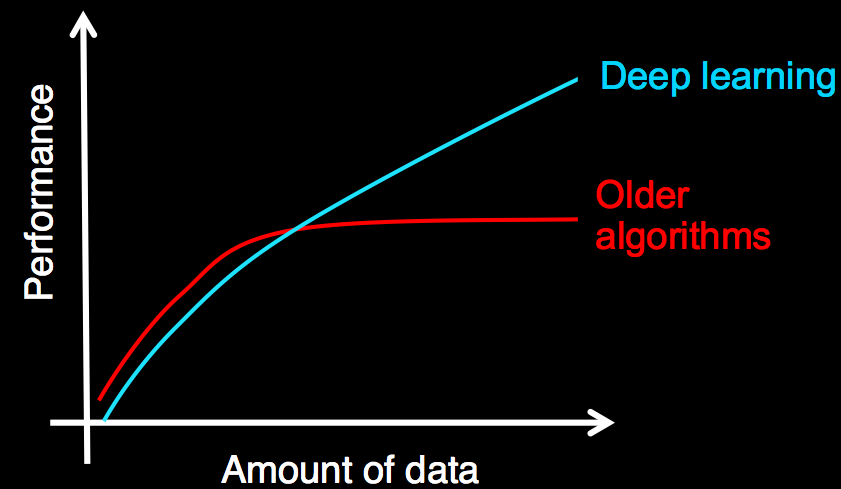
\includegraphics[width=0.4\textwidth]{figures/andrew-ng-big-data}\let\thefootnote\relax\footnotetext{\tiny{From Andrew Ng's CS229 Deep Learning slides (\url{http://cs229.stanford.edu/materials/CS229-DeepLearning.pdf})}}
\end{figure}
\begin{itemize}
\item Empirical observation: performance of deep neural networks has not plateaued with increasing amount of data.
\item Higher data throughput compared to other nonlinear methods.
\item Recent trends in system for ML: how to run (training/inference) large neural networks efficiently.
\end{itemize}
\note[item]{Theoretically, there is very little understanding why neural networks work. But one thing people tend to agree on is that they scale very well with large data.}
\note[item]{The empirical observation is that as we increase the amount of data, other learning algorithms plateaued, while the performance of neural networks keeps increasing. I don't have a reference to such a study; as you can see, the picture is cartoonish. However, all the big leading tech companies such as Google and Facebook has switched to many of their services to neural models, which means they must be superior to previous non-neural models at similar scales.}
\note[item]{The use of GPU and SGD with minibatches have made NN to have higher data throughput than other nonlinear methods.}
\note[item]{Many of its recent focus in SysML has been on how to train or do inference with neural network models more efficiently.}
\end{frame}

\begin{frame}
{Versatile architectures}
\begin{itemize}
\item Easy to incorporate inductive bias for different tasks.
\item Examples:
\begin{itemize}
\item Translation invariance in image recognition---convolution.
\item Dependence on past observations in time series---recurrence.
\item Alignment between input and (structured) output---attention.
\end{itemize}
\item Many building blocks can be composed together.
\end{itemize}
\note[item]{Another unique advantage of neural networks is that it's extremely versatile. Because of the compositional nature of NN architectures, it is very easy to incorporate inductive bias for different tasks.}
\note[item]{For examples, CNN is a very successful architecture for computer vision because it captures the translation invariance property of objects in images. A cat could appear anywhere in the image, so an effective representation must not depend on the location or scale of the object.}
\note[item]{RNN is popular for sequence problems where the observation at a certain time step depends on past observations, such as time series and word sequences.}
\note[item]{In structured prediction, we have seen that the output might depends on specific parts of the input. For example, in MT, French words in the output can be aligned to specific English words in the input. This alignment can be modeled by attentions.}
\end{frame}

\begin{frame}{Representation sharing}
\begin{itemize}
\item ``Classifiers'' are task-specific but representation/features can be shared.
\end{itemize}
\begin{center}
\def\layersep{2.5cm}
\begin{tikzpicture}[shorten >=1pt,->,draw=black!50, node distance=\layersep]
    \tikzstyle{every pin edge}=[<-,shorten <=1pt]
    \tikzstyle{neuron}=[circle,fill=black!25,minimum size=17pt,inner sep=0pt]
    \tikzstyle{input neuron}=[neuron, fill=green!50];
    \tikzstyle{output neuron}=[neuron, fill=red!50];
    \tikzstyle{hidden neuron}=[neuron, fill=blue!50];
    \tikzstyle{annot} = [text width=4em, text centered]

    % Draw the input layer nodes
    \foreach \name / \y / \text in {1/1/1, 2/2/2, 3/3/, 4/4/d-1, 5/5/d}{
    		\ifthenelse{\y=3}
    		{\node[input neuron, pin=left:$\vdots$] (I-\name) at (0,-\y) {}}
        {\node[input neuron, pin=left:$x_{\text}$] (I-\name) at (0,-\y) {}}
	;}
    % Draw the hidden layer nodes
    \foreach \name / \y in {1,...,4}
        \path[yshift=-.5cm]
            node[hidden neuron] (H-\name) at (\layersep,-\y cm) {};
            
    % Draw the hidden layer nodes
    \foreach \name / \y in {1,...,3}
        \path[yshift=-1cm]
            node[hidden neuron] (H2-\name) at (2*\layersep,-\y cm) {};

    % Draw the output layer node
    \node[output neuron,pin={[pin edge={->}]right:score 1}, above right=0.5cm and \layersep of H2-2] (O-1) {};
    \node[output neuron,pin={[pin edge={->}]right:score 2}, below right=0.5cm and \layersep of H2-2] (O-2) {};


    % Connect every node in the input layer with every node in the
    % hidden layer.
    \foreach \source in {1,...,5}
        \foreach \dest in {1,...,4}
            \path (I-\source) edge (H-\dest);
    \foreach \source in {1,...,4}
        \foreach \dest in {1,...,3}
            \path (H-\source) edge (H2-\dest);

    % Connect every node in the hidden layer with the output layer
    \foreach \source in {1,...,3}
    		\foreach \dest in {1,2}
        		\path (H2-\source) edge (O-\dest);

    % Annotate the layers
    \node[annot,above of=H-1, node distance=1.3cm] (hl) {{Hidden} layers};
    \node[annot,left of=hl] {Input layer};
    \node[annot,right of=hl, node distance=5cm] {Output layer};
    
\end{tikzpicture}
\end{center}
\note[item]{The last prominent advantage of NN we'll talk about today is representation sharing. Most models we've seen assume that the features are given and only learns the classifier, or the relation between the features and the output.}
\note[item]{In neural network, only the last layer is the ``classifier'', everything before can be considered as the representation, or the features. The classifier is task specific, but the representation can be shared across related tasks.}
\note[item]{Let's look at some instantiation of this idea.}
\end{frame}
%
\begin{frame}{Multitask Learning and transfer learning}
\begin{simpleblock}
{Multitask learning:}
\begin{itemize}
\item Learn related tasks together, \eg
\begin{itemize}
\item Object classification: cat or dog?
\item Object localization: location of the objects?
\end{itemize}

\item Basic features (\eg edges, texture) can be shared by tasks.
\begin{itemize}
\item Different output layers for each task; the rest is shared.
\item Objective function combines losses from both predictions, e.g. by averaging.
\end{itemize}
\end{itemize}
\end{simpleblock}

\onslide<2->{
\begin{simpleblock}
{Transfer learning:}
\begin{itemize}
\item Self-supervised \textbf{pre-training} to learn generic features.
\begin{itemize}
\item General idea: denoising, \ie perturbed input $\rightarrow$ original input.
\end{itemize}
\item On downstream tasks: \textbf{fine-tune} pre-trained models (reuse representation).
\end{itemize}
\end{simpleblock}
}
\note[item]{Suppose we want to do both object classification and localization. Obviously we need two classifiers as they don't even share the same output space.}
\note[item]{However, the basic image features can be useful to both tasks, such as detecting the edges and textures in a region of the image. So we can use the same representation learning layers for both tasks, and simply add one more output layer for the other task. This is the most basic version of transfer learning in NN.}
\note[item]{The other popular method based on representation sharing is pretrain-and-then-finetune. Suppose we don't have related tasks with annotation (note that to do multi-task learning we still need multiple annotated datasets). We can consider some self-supervised task as a task that is related to a family of tasks. For example, in NLP, language models can be considered as a task that is related to many other language problems.}
\note[item]{Most self-supervised tasks follow the denoising setup. You perturb your input, \eg mask a word in a sentence, and learn a model to recover the original input.}
\end{frame}
%
\begin{frame}
{Summary}
\begin{itemize}
\item Powerful use of features: representation learning
\item Fast and scalable with data given the right system support.
\item Hard to train: non-convex optimization
\begin{itemize}
\item Easier in practice with released code and libraries.
\end{itemize}
\item Gap exists between theory and practice:
\alarm{when and why does it work?}
\end{itemize}
\note[item]{Let's conclude now. The key idea in neural networks is representation learning. Instead of doing feature engineering, we can given the model raw features such as pixels and rely on it to discovers interesting patterns.}
\note[item]{We also covered backpropagation, which is basically partial derivatives and chain rule on a computation graph. But with SGD, it makes neural networks efficient to train with the right hardware.}
\note[item]{However, there is still so much unknown about neural networks. Why does SGD work? What's special about the hypothesis space of NNs? We have little theoretical understanding of these questions. To end on a more positive note, that also means that there are plenty of opportunities for you to make a contribution towards our understanding.}
\end{frame}


\end{document}
